\documentclass[a4paper, 12pt, titlepage]{article}

\usepackage[polish]{babel}	% Enable polish text
\usepackage[utf8]{inputenc}
\usepackage[T1]{fontenc}
\usepackage{times}
\usepackage{anysize}
\usepackage{amsmath}
\usepackage{soul} 			% Strike throught text (\st{}) 

\usepackage{hyperref} % Clickable table of contents
\hypersetup{colorlinks=true,
			allcolors=black,
			urlcolor=cyan}
\usepackage{enumitem} % noitemsep option in lists
\setlist{leftmargin=1.5cm, noitemsep}
\setlist[description]{labelindent=1.1cm, leftmargin=2cm}

\usepackage{datetime} % Enable currenttime  command
% advance the hour register by nr of hours
% negative values if you want to subtract
\advance\currenthour by 1

%\usepackage[none]{hyphenat} % Prevent hyphenation for words
\usepackage{ifthen}			% Enable ifthenelse function
\usepackage{graphicx}		% Enable pictures
\usepackage{alltt}			% Enable non-foramted text input

\marginsize{2cm}{2cm}{2cm}{2cm}


\title{Przetwarzanie obrazów cyfrowych\\
	Opracowanie pytań do egzaminu}
%\author{Vadym Perepeliak}


%%%%%%%%%%%%%%%%%
\begin{document}
\maketitle
\tableofcontents
\pagebreak
    
    
%%%%%%%%%%%%%%%%%%%%%%%%%%%%%%%%%%%%%%%%%%%%%%%%%%%%%%%%%%%%%%%%%%%%%%%%%%%%%%%%%%%%%%%
\pagebreak\section{Budowa oka i proces widzenia}

\subsection{Metody ekstrakcji (rozpoznania) tęczówki oka}
Filtry Gabora. \\
\includegraphics[scale=0.5]{identyfikacja_teczowki.png}

\subsection{Wymień elementy oka skupiające obraz na siatkówce}
Światło przechodzi przez rogówkę, źrenice regulowaną tęczówką – kolorową częścią oka, soczewkę, która załamuje promienie świetlne, ciało szkliste. Potem promienie padają na wewnętrzną warstwę oka – siatkówkę gdzie powstaje odwrócony obraz.

\subsection{Za co odpowiedzialne są pręciki w oku}
Pręciki mają wysoką czułość, przeznaczone do widzenia nocnego, odpowiedzialne za wykrywanie kształtu i ruchu. Brak czułości na barwę.

\subsection{Wymienić elementy siatkówki i punkty charakterystyczne na siatkówce}
Siatkówka składa się z fotoreceptorów – czopków (odpowiedzialne za kolor) i pręcików (odpowiedzialne za widzenie nocne), plamki żółtej – największe skupisko czopków oraz plamki ślepej – tam nie ma fotoreceptorów, od niej wychodzi nerw wzrokowy.

%%%%%%%%%%%%%%%%%%%%%%%%%%%%%%%%%%%%%%%%%%%%%%%%%%%%%%%%%%%%%%%%%%%%%%%%%%%%%%%%%%%%%%%
\pagebreak\section{Sztuczne systemy wizyjne}

\subsection{Podaj min. 3 cechy naturalnego przetwarzania obrazu przewyższające sztuczne przetwarzanie obrazu}
\begin{itemize}
	\item Szybka analiza złożonych obrazów
	\item Większa skuteczność rozpoznawania obrazów dwuznacznych
	\item Łatwe i efektywne uczenie się nowych schematów
	\item Szybsze rozpoznawanie obrazów w czasie rzeczywistym
\end{itemize}

\subsection{Podaj min. 3 cechy przewyższające sztuczne przetwarzanie obrazu}
\begin{itemize}
	\item Niższa cena analizy
	\item Szybszy czas reakcji
	\item Powtarzalność wyników
	\item Praca nie tylko w świetle widzialnym ale również np w podczerwieni
\end{itemize}

\subsection{Podaj dwie nowoczesne metody sztucznego przechwytywania obrazu i krótko je opisz. \\ 2 metody akwizycji obrazu w kamerach}
\begin{description}
	\item[Lampa analizująca] - stosowane zjawisko fotoelektryczne, w rezultacie powstaje obraz monochromatyczny. Zarejestrowanie kolorów wymaga współdziałania trzech lamp, do których jest doprowadzone światło rozbite na barwy podstawowe RGB.
	\item[CCD] (Układ ze sprężeniem ładunkowym) - półprzewodnikowa matryca złożona z milionów światłoczułych elementów (fotodiod). W poszczególnych diodach gromadzi się ładunek elektryczny, proporcjonalny do liczby padających fotonów.
\end{description}

\subsection{2 sposoby według których czujniki światła reagujące tylko na jego natężenie mogą rozróżniać kolory}
\begin{itemize}
	\item Specjalne filtry barwne, selektywnie dostarczające do poszczególnych pikseli jedną składową barwną $\rightarrow$ powstały obraz ma niższą jakość i rozdzielczość
	\item W układzie optycznym kamery światło rozszczepiane na składowe RGB, kierując go poprzez filtry widmowe na trzy elementy CCD $\rightarrow$ pewna rozdzielczość obrazu.
\end{itemize}

\subsection{Przyporządkuj parametry do standardów telewizyjnych. \\ NTSC i PAL wybrać odpowiednią ilość Hz i linii na pół-obrazie. \\ Liczba linii PAL, półobrazów i obrazów w czasie 1 sek}
\begin{description}
	\item[PAL] - 625 linii, 25 obrazów/s, częstotliwość odświeżania 50 Hz
	\item[NTSC] - 575 linii, 30 obrazów/s, częstotliwość odświeżania 60 Hz
\end{description}
	
\subsection{Czujniki CCD wykazują największą czułość dla fal...}
1050 nm - podczerwień
%%%%%%%%%%%%%%%%%%%%%%%%%%%%%%%%%%%%%%%%%%%%%%%%%%%%%%%%%%%%%%%%%%%%%%%%%%%%%%%%%%%%%%%
\pagebreak\section{Modele barw}

\subsection{Połącz przestrzenie barw z zastosowaniem}
\begin{description}[noitemsep, labelwidth=1.7cm]
	\item[CMY(K)] -	poligrafia (druk)
	\item[HSV] - w programach graficznych
	\item[RGB] - naturalne postrzeganie barw, ekran komputera i telewizora
	\item[YCrCb] - przesyłanie i przechowywanie wideo
	\item[YUV] - przesyłanie danych, analogowa TV (zgodność z czarno-białą - samo Y). Model YUV był wykorzystywany w czasie przechodzenia od telewizorów czarno-białych na kolorowe. Kamerka w smarfonie zapisuje w YUV
\end{description}

\subsection{Co to równomierna percepcyjnie przestrzeń barw (np CIE Lab) ?}
To taka przestrzeń barw, w której obszary różnicy percepcyjnej barw mają postać kul o jednakowym promieniu w obrębie całej przestrzeni barw. \par
Przestrzeń barw CIELab i CIELUV pretendują do miana równomiernych przestrzeni barw jednak faktycznie są jej przybliżeniem. (\href{https://pl.wikipedia.org/wiki/R%C3%B3wnomierna_przestrze%C5%84_barw}{link do Wikipedii})
	
\subsection{Opisać CIE Lab}
\textbf{CIELab} – przestrzeń barw, która została znormalizowana w 1976 przez CIE (Międzynarodową Komisję Oświetleniową). Barwę opisują matematycznie trzy składowe: L - jasność (luminancja), a – barwa od zielonej do magenty, b – barwa od niebieskiej do żółtej.
	
\subsection{Kodowanie CMYK a CMY. \\ Co to K w modelu CMY/CMYK}
CMY(Cyan, Magenta(purpurowy), Yellow) - subtraktywny model barwny.
Z powodu niedoskonałości tuszów stosowanych w urządzeniach do druku, dodając takie same ilości kolorów CMY, nie uzyskamy głębokiej czerni, tylko w większości przypadków kolor ciemno brązowy. Aby zlikwidować ten problem, do zestawu kolorów CMY sdecydowano dodać barwę czarną K = min(C, M, Y).\par
K to minimum z C, M i Y albo osobny kolor czerni.

\subsection{Czerwony w YCrCb zawarty jest w…}
Odp: Cr. Y\textquoteright~is the luma component and Cb and Cr are the blue-difference and red-difference chroma components.

\subsection{Jakie wartości w CMY dadzą kolor niebieski}
C(255) M(255) Y(0) \\
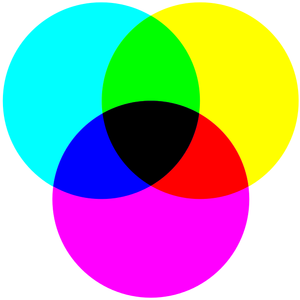
\includegraphics[scale=0.8]{CMY_ideal.png}

\subsection{Kodowanie CMY(jak otrzymać z RGB)}
$\begin{bmatrix} C \\ M \\ Y \\ \end{bmatrix} 
= \begin{bmatrix} 1 \\ 1 \\ 1 \\ \end{bmatrix}
- \begin{bmatrix} R \\ G \\ B \\ \end{bmatrix} $

\subsection{Czym jest Y w YUV.}
Y – luminacja (dla obrazu monochromatycznego), U – składowa niebieska, V – składowa czerwona.

%%%%%%%%%%%%%%%%%%%%%%%%%%%%%%%%%%%%%%%%%%%%%%%%%%%%%%%%%%%%%%%%%%%%%%%%%%%%%%%%%%%%%%%
\pagebreak\section{Rozdzielczość i skalowanie}

\subsection{Czym się różni Nearest Neighbour od interpolacji}
W metodzie Nearest Neighbour brany jest pod uwagę tylko jeden najbliższy piksel. W metodzie interpolacji brane pod uwagę są piksele otoczenia np. 8 pikseli dla okna 3x3.

\subsection{Skalujemy obraz sztuczny przedstawiający szachownicę do wyższej rozdzielczości. Stosujemy metodę najbliższego sąsiada oraz metodę interpolacji. Która metoda będzie lepsza i dlaczego?}
Lepsza będzie metoda najbliższego sąsiada, która dla obrazów z niewielką ilością stopni szarości (sztucznych) nie powoduje zniekształceń wynikających z uwzględniania otoczenia piksela jak w metodzie interpolacji.

\subsection{Mamy czarno-białą kratownice i ją powiększamy. Stosujemy metodę najbliższego sąsiada oraz metodę interpolacji. Która metoda będzie lepsza i dlaczego?}
Wyniki będą podobne dla czarno-białego obrazu. Jednak metoda interpolacji może dać lepszy obraz ze względu na linii inne od poziomych i pionowych, ponieważ jest brana pod uwagę otoczenie piksela.

\subsection{Co to jest 720p}
Termin ten wskazuje, że obraz ma 720 linii poziomych. W formacie 16:9 jest to
obraz o wymiarach 1280x720. Literka ‘p’ wskazuje, że obraz jest bez przeplotu.

\subsection{Co to jest 1080i}
Określa rozdzielczość obrazu równą 1920x1080. Literka ‘i’ wskazuje, że obraz jest z przeplotem (naprzemienne wyświetlanie parzystych i nieparzystych linii obrazu). \par
Literka p - \textbf{progressive scan} czyli wyświetlane we wszystkich klatkach pełne obrazy. Literka i - \textbf{interlaced} czyli z przeplotem wyświetlane są pół-obrazy. Lepsze jest z \textbf{p}.

%%%%%%%%%%%%%%%%%%%%%%%%%%%%%%%%%%%%%%%%%%%%%%%%%%%%%%%%%%%%%%%%%%%%%%%%%%%%%%%%%%%%%%%
\pagebreak\section{Przekształcenia obrazu}

\subsection{2 metody normalizacji}
\begin{description}[noitemsep]
	\item[Skalowanie z obcięciem] - dodajemy/odejmujemy pewną wartość i usuwamy wartości poza zakresem.
	\item[Skalowanie bez obcięcia] dodajemy/odejmujemy najmniejszą wartość a następnie dzielimy wszystko tak by największa wartość była równa maksymalnej możliwej wartości
\end{description}

\subsection{Opisać operację LUT}
Operacja korzysta z gotowych tabel przekodowania look-up tables, w których dla każdej wartości piksela oryginalnego obrazu mamy gotową wartość piksela nowego obrazu.

\subsection{Wybrać operacje bezkontekstowe}
Operacje bezkontekstowe: LUT, negacja, binaryzacja (globalna), wyrównanie histogramu, dodawanie, odejmowanie, mnożenie, \st{filtr morfologiczny}, \st{mediana}

\subsection{Jak zrobić przekształcenie punktowe nie mając danego przepisu analitycznego}
???

\subsection{Coś o współczynnikach normalizacji w maskach - dla podanych masek 3x3 podać ich współczynniki normalizacyjne}
Współczynnik normalizacji W to jest suma wag w masce.
$$ W = \sum w(i,j) $$
Dla maski: 
\begin{tabular}{|c|c|c|}
	\hline
	1 & 4 & 1 \\ \hline
	4 & 3 & 4 \\ \hline
	1 & 4 & 1 \\ \hline
\end{tabular} W = 23 
%%%%%%%%%%%%%%%%%%%%%%%%%%%%%%%%%%%%%%%%%%%%%%%%%%%%%%%%%%%%%%%%%%%%%%%%%%%%%%%%%%%%%%%
\pagebreak\subsection{Histogram obrazu}

\subsection{Opisać krótko algorytm wyrównywania histogramu (HE)}
Etapy równoważenia histogramu:
\begin{enumerate}
	\item Obliczenie histogramu skumulowanego (suma pikseli dla poszczególnych poziomów szarości + suma poprzednich poziomów).
	\item Normalizacja histogramu skumulowanego (dzielenie przez sumę pikseli).
	\item Pomnożenie wartości otrzymanych w pkt.2 przez maksymalną wartość poziomu szarości i zaokrąglenie do liczb naturalnych.
	\item Utworzenie obrazu wynikowego poprzez przypisanie pikselom na poszczególnych poziomach szarości nowych wartości wyliczonych w poprzednich krokach.
\end{enumerate}


\subsection{Histogram BBHE i DISHE, czym się charakteryzują i po co są \\ Dlaczego metody BBHE i DISHE są lepsze od klasycznego wyrównywania histogramu HE?}
Klasyczne wyrównywanie histogramu HE ma jedną zasadniczą wadę: po wykonaniu operacji
jasność obrazu ulega zmianie. Metody, które eliminują to niekorzystne zjawisko polegają na dekompozycji obrazu wejściowego na dwa podobrazy (wg. pewnego kryterium) i wykonania operacji HE dla tych podobrazów. 
\begin{description}
	\item[BBHE] (Bi-Histogram Equalization) - kryterium podziału to średnia jasność w obrazie.
	\item[DSIHE] (Dualistic Sub-Image Histogram Equalization) - obraz dzielony jest na dwa podobrazy o takiej samej ilości pikseli (jaśniejszych i ciemniejszych) 
\end{description}

%%%%%%%%%%%%%%%%%%%%%%%%%%%%%%%%%%%%%%%%%%%%%%%%%%%%%%%%%%%%%%%%%%%%%%%%%%%%%%%%%%%%%%%
\pagebreak\section{Binaryzacja}

\subsection{Jedna metoda znajdowania progu binaryzacji + opis}
Próg binaryzacji możemy znaleźć analizując histogram obrazu. Na ogół będziemy mieć do czynienia z dwiema “górkami” pikseli - jedna to piksele obiektu, drugie tła (jasne obiekty na ciemnym tle lub na odwrót). Próg dobieramy biorąc wartość pomiędzy nimi, w dolinie. Pozwoli to na oddzielenie obiektów od tła.

\subsection{Znajdowanie progu binaryzacji metodą histerezy + opis \\ Wyjaśnij na czym polega binaryzacja z histerezą}
Progowanie z histerezą stosuje się w przypadkach, gdy klasy pikseli w histogramie nie są wyraźnie rozseparowane, np. gdy granice obiektu w obrazie są rozmazane, niewyraźne. W takim przypadku definiuje się dwa progi: lewy oraz prawy. Wartości leżące poniżej progu lewego definiują część główną obiektu, wartości leżące powyżej progu prawego wyznaczają tło. Wartości między lewym a prawym progiem są klasyfikowane jako reprezentujące obiekt pod warunkiem, że piksel przyjmujący taką wartość sąsiaduje w obrazie z pikselem należącym do głównego obiektu.\\
% TODO: przerobić na latex
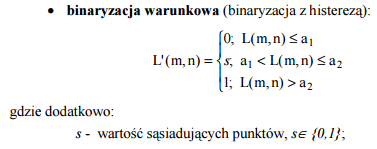
\includegraphics[scale=0.8]{Bin_histereza_wzor.png} 
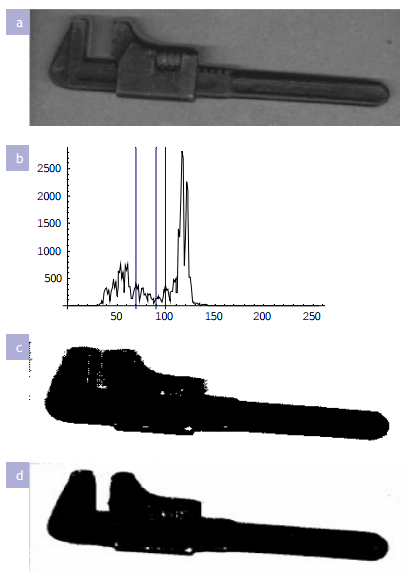
\includegraphics[scale=0.8]{Bin_histereza.png}

\subsection{Ryż na obrazku się źle zbinaryzował (jakieś plany czarne itp) i trzeba napisać jak się tego pozbyć (wykorzystano metodę Savouli)}
???

\subsection{Podaj przykład metody automatycznego wyznaczania progu binaryzacji. Na podstawie czego jest wyznaczany?}
\begin{description}[noitemsep]
	\item[Ots'u] - automatycznie testuje się różne progi i szuka takiego progu, dla którego wariancja międzygrupowa będzie najwyższa a wariancja wewnątrzgrupowa będzie najniższa. Wynik uzyskujemy poprzez analizę średnich ważonych w komponentach.
	\item[Yen] - maksymalizacja entropii obiektów i tła
	\item[Kittler] - podobnie jak Ots'u, tylko liczona jest dystrybuanta prawdopodobieństwa i odchylenie	standardowe

\end{description}

\subsection{Kiedy używa się binaryzacji lokalnej}
W przypadku niejednorodnie oświetlonego obrazu.\\
Krótki opis binaryzacji lokalnej:
\begin{enumerate}[noitemsep]
	\item Podziel obraz na rozłączne kratki np. 8x8 pikseli
	\item W każdej kratce wyznacz próg binaryzacji (np. za pomocą Otsu)
	\item Dla każdego piksela użyj lokalnego progu, który jest przybliżony za pomocą 4 najbliższych progów.
\end{enumerate}
%%%%%%%%%%%%%%%%%%%%%%%%%%%%%%%%%%%%%%%%%%%%%%%%%%%%%%%%%%%%%%%%%%%%%%%%%%%%%%%%%%%%%%%
\pagebreak\section{Filtracja kontekstowa}

\subsection{Filtracja kontekstowa - opisać}
Oznacza że dla wyznaczenia wartości jednego punktu obrazu wynikowego trzeba dokonać obliczenia na wielu punktach obrazu oryginalnego, z reguły na punktach sąsiednich.

\subsection{Dlaczego w filtracji górnoprzepustowej nie stosuje się normalizacji tak jak w filtracji dolnoprzepustowej?}
Jeżeli chodzi o maskę: w górnoprzepustowych pomija się normalizację, czyli dzielenie przez sumę wag, bo $suma~wag = 0$. \\
Jeżeli chodzi o wynikowy obraz: w filtracji górnoprzepustowej \st{nie} stosuje się normalizacji dlatego, że mogą tam występować ujemne współczynniki wag, stąd wartości pikseli mogą wykroczyć poza zakres 0 - 255.

\subsection{Jak działa filtr medianowy? \\ Podany obraz, jak będzie wyglądał środkowy piksel po filtracji medianowej?}
Bierze pod uwagę środkową wartość (medianę) uporządkowanych pikseli z otoczenia rozważanego piksela. Ekstremalne wartości nie wpływają na jego działanie. Bardzo skutecznie zwalcza szumy, nie powodując ich rozmazywania na większym obszarze. Nie wprowadza do obrazu nowych wartości, więc obraz po filtracji nie wymaga skalowania. Nie powoduje pogorszenia ostrości krawędzi, ale ma tendencję do zjadania narożników.

\subsection{Czy filtr medianowy z oknem 5x5 całkowicie odfiltruje zakłócenia o (ciemne zakłócenie na jasnym tle) dla zakłócenia o rozmiarze: 2x4, 3x5, 6x5, 2x14?}
Będą odfiltrowane zakłócenia tylko o rozmiarach 2x4 i 2x14, bo brana jest media ze wszystkich punktów otoczenia. Ilość punktów zakłócenia w oknie ma być mniejsza niż $\frac{5\times5}{2}\approx12$.

\subsection{Za pomocą, których masek można otrzymać filtr kombinowany \\ Jakie gradienty można zastosować w filtrach kombinowanych \\ Jakie filtry mogą być kombinowane}
Za pomocą dwóch prostopadłych (w różnych kierunkach) masek Sobela (Prewitta) i kombinacji Euklidesowej lub modułowej. Nazywane: "gradient Sobela", "gradient Prewitta", "gradient Kirscha" (nie był omawiany ale istnieje). \\
Kombinacja Euklidesowa:
$$ L^{\prime}(m,n) = \sqrt{(L_{1}(m,n))^2+(L_{2}(m,n))^2} $$
Uproszczona formuła modułowa:
$$ L^{\prime}(m,n) = |(L_{1}(m,n)|+|L_{2}(m,n)| $$

\subsection{Filtracja adaptacyjna - opisać \\ Co wykrywa filtr adaptacyjny w pierwszym etapie działania? \\ Jaki jest drugi etap jego działania? \\ W jakim celu może być zastosowany filtr adaptacyjny?}
Filtry adaptacyjne zmieniają charakterystykę działania w zależności od cech analizowanego obrazu. Filtry te działają dwuetapowo:
\begin{enumerate}[noitemsep]
	\item W pierwszym etapie wyznaczamy czy należy dany punkt do krawędzi. Jako kryterium można przyjąć różnice stopni szarości w jego otoczeniu.
	\item Dokonuje się filtracji filtrem uśredniającym ale tylko dla punktów które nie należą do krawędzi. Punkty krawędzi pozostają bez zmian.
\end{enumerate}
Zastosowania:
\begin{itemize}[noitemsep]
	\item Wyrównanie intensywności poszczególnych płaszczyzn nie rozmazując krawędzie.
	\item Wzmocnienie krawędzi bez niepotrzebnych szczegółów w jednolitych obszarach.
\end{itemize}

\subsection{Wybrać filtr liniowy z podanych}
Filtry liniowe: Uśredniający, Robertsa, Prewitta, Sobela, Laplasjany

\subsection{Zaproponuj maskę do wykrycia krawędzi poziomych}
Maska Sobela:
\begin{tabular}{|c|c|c|}
	\hline
	1 & 2 & 1 \\ \hline
	0 & 0 & 0 \\ \hline
	-1 & -2 & -1 \\ \hline
\end{tabular}
\subsection{Podaj przykład maski wykrywające krawędzie pionowe}
Maska Sobela:
\begin{tabular}{|c|c|c|}
	\hline
	1 & 0 & -1 \\ \hline
	2 & 0 & -2 \\ \hline
	1 & 0 & -1 \\ \hline
\end{tabular}

\subsection{Maska 3x3 wykrywająca krawędzie pionowe + zaznaczenie na obrazie wynikowym krawędzi wykrytej + zastosowanie filtracji medianowej 3x3}
Maska Sobela wykrywajace krawędzie pionowe:
\begin{tabular}{|c|c|c|}
	\hline
	1 & 0 & -1 \\ \hline
	2 & 0 & -2 \\ \hline
	1 & 0 & -1 \\ \hline
\end{tabular}.
Filtracja medianowa: Bierze pod uwagę środkową wartość (medianę) uporządkowanych pikseli z otoczenia rozważanego piksela.

\subsection{Jaka maska z podanych wyostrzy krawędzie}
Przykładowe maski laplasjany do wykrywania krawędzie:
\begin{tabular}{|c|c|c|}
	\hline
	0 & -1 & 0 \\ \hline
	-1 & 4 & -1 \\ \hline
	0 & -1 & 0 \\ \hline
\end{tabular}
\begin{tabular}{|c|c|c|}
	\hline
	-1 & -1 & -1 \\ \hline
	-1 & 8 & -1 \\ \hline
	-1 & -1 & -1 \\ \hline
\end{tabular}

\subsection{Podana zlogarytmowana wizualizacja amplitudy jakiegoś filtra. Jaki to filtr? dolnoprzepustowy górnoprzepustowy, zaporowy?}
???

\subsection{Obraz Lena z samymi krawędziami, która filtracja wykonana: dolnoprzepustowa, górnoprzepustowa, przemnożenie przez stałą}
Racej górnoprzepustowa skoro są same krawędzie.

\subsection{Z czego składa się filtr gabora}
???

\subsection{Wykres 3D filtra, jaki to filtr: dolnoprzepustowy, górno-, środkowozaporowy, środkowoprzepustowy}
???

\subsection{Różnice pomiędzy filtracją bilateralną a non local means}
Filtracja bilateralna polega na tym, że wartość piksela zastępuje się bardzo specjalną średnią z pikseli otoczenia analizowanego piksela. Nie jest to zwykła średnia arytmetyczna, lecz średnia ważona, w której wagami są zarówno odległość piksela otoczenia od badanego piksela, ale także różnica w cechach radiometrycznych np. intensywności. W efekcie tego zachowane są ostre krawędzie. 
Filtracja non-local means robi tak samo ale uśrednianie obejmuje większy obszar pikseli (np. 20x20).

\subsection{Jak uogólnić funkcję bilateralną dla obrazów w kolorze?}
Odpowiednio zdefiniować odległość pomiędzy pikselami, która służy jako dodatkowa waga w uśrednianiu. 

\subsection{Czym jest dekonwolucja obrazu?}
Proces odwrotny do splotu funkcji. Polega na określeniu funkcji określającej zakłócenia w celu ich
odfiltrowania od zarejestrowanych danych. Przykładowe metody dekonwolucji: filtr odwrotny, filtr pseudoodwrotny, filtr Wienera, niewidomej dekonwolucji.

\subsection{Przykład operacji: kontekstowej liniowa, punktowej dwuargumentowej i 2x punktowa jednoargumentowa}
\begin{description}[noitemsep]
	\item[Kontekstowa liniowa] - filtr górnoprzepustowy
	\item[Punktowa dwuargumentowa] - dodawanie obrazów
	\item[Punktowe jednoargumentowe] - negacja, LUT

\end{description}

\subsection{Jaka wartosc będzie miał piksel po przefiltrowaniu medianowym z maską krzyżową (był podany wycinek obrazu)}
Chyba chodzi o operator krzyżyowy Robertsa, czyli najpierw filtrujemy maską 
\begin{tabular}{|c|c|}
	\hline
	0 & 1 \\ \hline
	-1 & 0 \\ \hline
\end{tabular} a potem
\begin{tabular}{|c|c|}
	\hline
	1 & 0 \\ \hline
	0 & -1 \\ \hline
\end{tabular} i na końcu liczymy z pikseli obu wynikowych obrazów pierwiastek z sumy kwadratów (ombinacja Euklidesowa). 


%%%%%%%%%%%%%%%%%%%%%%%%%%%%%%%%%%%%%%%%%%%%%%%%%%%%%%%%%%%%%%%%%%%%%%%%%%%%%%%%%%%%%%%
\pagebreak\section{Przekształcenia morfologiczne}

\subsection{Jako jaki filtr można traktować dylatację}
Filtr maksymalny.

\subsection{Jako jaki filtr można traktować erozję}
Filtr minimalny.

\subsection{Ustaw w ciąg rosnący wg. wielkości pól: figurę wejściową f oraz figury otrzymane po podstawowych przekształceniach morfologicznych dylatacji D(f), erozji E(f), zamknięcia Z(f) i otwarcia O(f)}
E(f) < O(F) < f < Z(f) < D(f)

\subsection{Co wykryje Bottom-Hat}
Minima lokalne obrazu (obszary lokalnie najciemniejsze)

\subsection{Co wykryje Top-Hat}
Maksima lokalne obrazu (obszary lokalnie najjaśniejsze)

\subsection{Jak wykorzystać operacje otwarcia/zamknięcia do wyszukiwania lokalnych ekstremów}
Maksima: Otwarcie - oryginał, binaryzacja z dolnym progiem
Minima: Zamknięcie - oryginał, binaryzacja z dolnym progiem

\subsection{Ścienianie definicja + przykład}
Ścienianie obiektu X przy użyciu el. strukturalnego B polega na przyłożeniu tego elementu do każdego punktu obrazu tak, aby punkt centralny pokrywał się z tym punktem i albo nie zmieniać wartości punktu jeśli element nie pokrywa się z jego sąsiedztwem albo zmienić wartość na \textbf{0} jeśli się pokrywa.

\subsection{Co to jest operacja pogrubiania. Podaj przykład}
Ścienianie obiektu X przy użyciu el. strukturalnego B polega na przyłożeniu tego elementu do każdego punktu obrazu tak, aby punkt centralny pokrywał się z tym punktem i albo nie zmieniać wartości punktu jeśli element nie pokrywa się z jego sąsiedztwem albo zmienić wartość na \textbf{1} jeśli się pokrywa. \\
Przykład: ???

\subsection{Obcinanie gałęzi}
Polega na stopniowym redukowaniu odcinków posiadających wolne zakończenie. Można traktować jako ścienianie przy elemencie strukturalnym:
\begin{tabular}{|c|c|c|}
	\hline
	0 & x & x \\ \hline
	0 & 1 & 0 \\ \hline
	0 & 0 & 0 \\ \hline
\end{tabular}


\subsection{Wypisać etapy wypełniania dziur}
\begin{enumerate}[noitemsep]
	\item Wyznaczenie negatywu z obrazu wyjściowego
	\item Wyczyszczenie brzegu negatywu(w wyniku tego pozostają na obrazie same otwory)
	\item Wyznaczenie operacji $OR$ obrazu wyjściowego i wyniku z punktu 2
\end{enumerate}
Przykład: \\
\begin{center}
	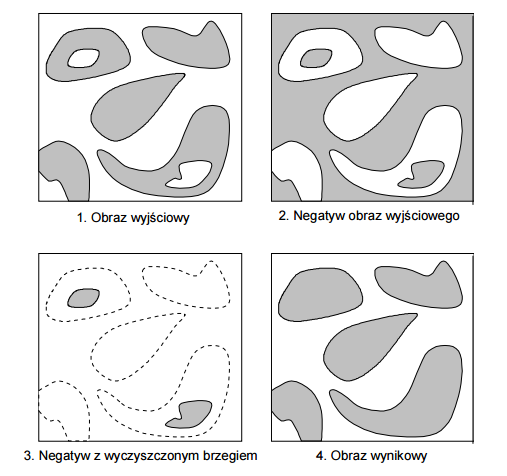
\includegraphics[scale=1]{wypelniania_dziur.png}
\end{center}

\subsection{Która maska to szkieletyzacja}
Szkieletyzacja może być realizowana jako ścienanie z elementem strukturalnym: 
\begin{tabular}{|c|c|c|}
	\hline
	x & 0 & x \\ \hline
	x & 1 & x \\ \hline
	1 & 1 & 1 \\ \hline
\end{tabular} 
\begin{description}[noitemsep]
	\item[0] piksel o szarości mniejszej od tła
	\item[1] piksel o szarości większej od tła
	\item[x] piksel o dowolnej szarości
\end{description}

\subsection{Opisać operację czyszczenie brzegu}
Ma na celu usunięcie z obrazu wszystkich obszarów, które przecinają brzeg obrazu. Przydaje się jak chcemy dokonać jakiejś operacji wyłącznie na w pełni widocznych obiektach. \par
Algorytm:
\begin{enumerate}[noitemsep]
	\item Tworzenie markerów (wspólnej części obrazu i jego brzegu)
	\item Rekonstrukcja obiektów przeciętych przez brzeg obrazu
	\item Generacja różnicy obrazu wejściowego i obrazu z obiektami po rekonstrukcji
\end{enumerate}

\subsection{Opisać rekonstrukcję}
Cykliczna dylatacja obrazu i wyznaczanie części wspólnej (operacja $AND$)z obrazu po dylatacji oraz wyjściowego całego przekształcenia - usuwa się fragmenty, które “wyszły” poza figurę.

\subsection{Wyznaczanie centroidów jest wykonywane za pomocą operacji}
Ścienianie przy użyciu dwóch elementów strukturalnych:
\begin{tabular}{|c|c|c|}
	\hline
	0 & x & x \\ \hline
	0 & 1 & 1 \\ \hline
	0 & 0 & x \\ \hline
\end{tabular} 
\begin{tabular}{|c|c|c|}
	\hline
	x & 0 & x \\ \hline
	0 & 1 & 1 \\ \hline
	x & 0 & x \\ \hline
\end{tabular} 

%%%%%%%%%%%%%%%%%%%%%%%%%%%%%%%%%%%%%%%%%%%%%%%%%%%%%%%%%%%%%%%%%%%%%%%%%%%%%%%%%%%%%%%
\pagebreak\section{Transformacja Hougha}
\subsection{Jakie niepożądane efekty powstają w przekształceniu Hougha do przestrzeni A,B? Jak temu zapobiec?} ???
Jeżeli linia jest pionowa, to wspolczynnik $a$ dochodzi do nieskończoności, co bardzo utrudnia obliczenia.

\section{Były podane dwa punkty o współrzędnych (0,0)(0,0) i (1,1)(1,1). Podaj wzór na prostą i narysuj ich interpelację w przestrzeni Hougha.}
Wzór na prostą:
$$ y=a\cdot x+b $$
$$ 0=a\cdot 0+b $$
$$ 1=a\cdot 1+b $$
Teraz zamieniam to na: $b = 0 (dla~kazdego~a)$ oraz $a = 1 - b$ i to są proste ilustrujące każdy z tych punktów w przestrzeni Hougha. Przecinają się w punkcie $a = 1, b = 0$ i ten punkt reprezentuje prostą łączącą te 2 punkty.

\subsection{Transformata Hougha dla dwóch pikseli}
???

%%%%%%%%%%%%%%%%%%%%%%%%%%%%%%%%%%%%%%%%%%%%%%%%%%%%%%%%%%%%%%%%%%%%%%%%%%%%%%%%%%%%%%%
\pagebreak\section{Segmentacja}

\subsection{Etapy segmentacji (przez podział)}
\begin{enumerate}[noitemsep]
	\item Ustalenie testu jednolitości
	\item Podzielenie obrazu na obszary o takich samych rozmiarach
	\item Zastosować test dla każdego regionu
	\item Jeśli obszar jest jednolity, to należy zlepić go z sąsiadami
	\item Jeśli nie spełnia, to ponownie podzielić
	\item Proces kontynuować aż wszystkie obszary zdadzą test
\end{enumerate}


\subsection{Segmentacja przez podział obszaru - co to jest i podać 2 problemy jakie przy niej występują.}
Dzieli się stopniowo obszary na mniejsze dopóki wszystkie ich piksele mają własności znacznie różniące się od tych w innych obszarach.  \\
Problemy:
\begin{enumerate}[noitemsep]
	\item Wybór progu jednolitości
	\item Powstawanie fałszywych obiektów (izolowane punkty o wartości 1 gdy dookoła są wyłącznie punkty tła)
\end{enumerate}

\subsection{Segmentacja przez rozrost}
Szuka się grup elementów o zbliżonej własności, zaczynamy od jednego elementu i sprawdzamy, czy są podobne, jeśli tak, to je grupujemy razem.

\subsection{Segmentacja metodą wykrywania krawędzi}
Szukamy granic pomiędzy obszarami, które niebezpośrednio definiują obiekt. Najpierw znajdujemy piksele, które mogą należeć do krawędzi, a potem zlepiamy je do pojedynczych segmentów linii, które z kolei też są łączone i tworzą granice obiektu. Używa się gradientów Sobela, Prewitta itd.

\subsection{Segmentacja oparta na statystyce}
Stosujemy kiedy segmenty są wypełnione jakimś stałym wzorcem (teksturą), pojedyncze obszary znacznie różniące się od siebie stanowią jeden obszar.

\subsection{Dlaczego cienie stanowią problem dla metody segmentacji z generacją tła}
Cienie spełniają wszystkie warunki, aby być kwalifikowane jako obiekty pierwszego planu, ale z punktu widzenia analizy obrazów można go uznać za zakłócenie, więc utrudnia analizę.

\subsection{Czy segmentacja obiektów pierwszoplanowych to segmentacja obiektów ruchomych. Uzasadnić}
Nie, obiekty pierwszoplanowe, to te które są dla nas interesujące, może to być np. człowiek, który cały czas leży. Jednocześnie może być wiele obiektów ruchomych, które są tłem(np. powiewające gałęzie drzewa).

\subsection{Dlaczego model statycznego tła nie sprawdza się w metodzie segmentacji z generacją tła?}???


\subsection{Czy metoda aktywnego konturu będzie działać dla pisma ze starodruku.}
Nie, ponieważ nie poradzi sobie z “wewnętrznymi dziurami” w literach.
%%%%%%%%%%%%%%%%%%%%%%%%%%%%%%%%%%%%%%%%%%%%%%%%%%%%%%%%%%%%%%%%%%%%%%%%%%%%%%%%%%%%%%%
\pagebreak\section{Indeksacja}

\subsection{Indeksacja jednoprzebiegowa - napisać po co i gdzie się stosuje}
Można zaoszczędzić czas obliczeń, szczególnie dla obrazów z niewielką liczbą obiektów oddalonych od siebie, znajduje zastosowanie w potokowym przetwarzaniu strumienia wizyjnego za pomocą układu FPGA.

\subsection{Opisz drugą iterację w drugim przebiegu indeksacji}
Algorytm:
\begin{enumerate}[noitemsep]
	\item Przeglądanie zbinaryzowanego obrazu linia po linii aż do napotkania punktu o wartości 1, wtedy nadaje mu się etykietę, analizując jego otoczenie i zapisując w tablicy sklejeń. 
	\item W drugiej iteracji tablica sklejeń może w prosty sposób zostać użyta do przeindeksowania źle zaindeksowanych części obiektów, można ją użyć jako podstawę do operacji LUT.
\end{enumerate}

\subsection{Czego dotyczy formuła croftona}
Pomiaru długości brzegu figury. Jest to formuła Cauchy’ego po przekształceniu.

\subsection{Metody ramki bezpieczeństwa wykorzystuje się przy pomiarach ...} Liczebności elementów
%%%%%%%%%%%%%%%%%%%%%%%%%%%%%%%%%%%%%%%%%%%%%%%%%%%%%%%%%%%%%%%%%%%%%%%%%%%%%%%%%%%%%%%
\pagebreak\section{Transformata Fouriera}

\subsection{Czym jest F(0,0)}
Element o indeksach (0,0) w dziedzinie Fouriera i jest sumą wszystkich wartości dwuwymiarowego ciągu L, czyli obrazu.

- Jak można wykorzystać transformatę fouriera do rozpoznawania kształtów


- Jaki wpływ na F-obraz ma filtr Hamminga/Chebysheva/jakieś dwa inne zamiast standardowego (idealnego)?
Od typu okna zależy różnice pomiędzy widmem sygnału obserwowanego, a widmem wyniku obserwacji.

- Filtracja w dziedzinie częstotliwości
Mnożenie całego obrazu przez maskę.
Filtracja w dziedzinie F-obrazu może okazać się bardziej efektywna od klasycznej konwolucji (np. dla dużego obrazu z dużą maską).
Zastosowania:
Wykrywanie dominującej orientacji, usuwanie zakłóceń okresowych, usuwanie rozmazania wynikającego z ruchu, wyszukiwanie wzorca i korelacja

- Filtracja w dziedzinie F-obrazu
Mnożenie punktowe dwóch F-obrazów, jednego pochodzącego od filtrowanego obrazu i drugiego będącego filtrem.
Filtracja dolnoprzepustowa: zachowuje się elementy F-obrazu w środku
Filtracja górnoprzepustowa: zachowuje się elementy F-obrazu na zewnątrz
Schemat:
Wyznaczenie transformaty Fouriera obrazu
Wymnożenie F-obrazu przez funkcję filtru
Wyznaczenie transformaty odwrotnej

- Po co się logarytmuje amplitudę w fourierze
W celu lepszej wizualizacji(?)
Dokładniej w celu zmniejszenia dysproporcji między składową stałą (F(0,0)), która ma wartości duże, a składowymi częstotliwościowymi, które przyjmują niewielkie wartości

- Fourier splotu odpowiada czemu
Jest to operacja równoważna filtracji w dziedzinie F przy założeniu okresowości obrazu

- Czemu FFT w dwóch krokach liczyć (2x 1D)
Ułatwia obliczenia(możemy traktować jako ciągi jednowymiarowe)

- Jak się robi splot 2d


- Po co stosuje się przesunięcie w transformacie Fouriera?
Dla wygodniejszej analizy, wtedy niskie częstotliwości są w środku F-obrazu.
%%%%%%%%%%%%%%%%%%%%%%%%%%%%%%%%%%%%%%%%%%%%%%%%%%%%%%%%%%%%%%%%%%%%%%%%%%%%%%%%%%%%%%%
\pagebreak\section{DCT JPEG}
- dwa tryby liczenia DCT w DV i kiedy który


- kodowanie DV etapy i metody


- Jeśli DC jest dodatni a AC są zerami to obraz będzie: czarny, w odcieniach szarości, jednolity, inny
czarny, jednolity

- Jakie cechy ludzkiego wzroku wykorzystuje JPEG (min 2.)
mniejsza rozdzielczość widzenia kolorów niż jasności
mała wrażliwość na amplitudę szybkich zmian jasności

- Współczynniki AC i DC w DCT mogą być …
DC - wyłącznie nieujemne,
AC - dowolne


- Etapy dekompresji JPEG. Zaznaczyć które to dekompresja a które to przekształcenie.
Huffman - dekompresja
RLE - dekompresja
Utworzenie bloków 8x8 dla każdego z kanałów YUV - przekształcenie
ZigZag - przekształcenie
Dekwantyzacja na każdym bloku - dekompresja


- Opisać etapy kompresji JPEG i każdy z nich przyporządkować do: przekształcenia, kompresji stratnej i kompresji bezstratnej

RGB -> YUV - przekształcenie
DCT - przekształcenie
kwantyzacja - kompresja stratna
Zig-Zag - przekształcenie
kodowanie RLE - kompresja bezstratna
kodowanie Huffmana - kompresja bezstratna

- Wymień poziomy MPEG-2 
wysoki, wysoki typu 1440,  główny,  niski

- Wyjaśnij na czym polega kodowanie międzyramkowe sekwencji wideo, podaj przykład standardu, który wykonuje tą metodę. 
Przy kodowaniu międzyramkowym sekwencja wizyjna składa się z ramek kluczowych zawierających pełny obraz. Pomiędzy ramkami kluczowymi znajdują się ramki delta, w których zakodowane są tylko różnice przyrostowe. Zapewnia to często znaczny stopień kompresji, ponieważ w wielu sekwencjach ruchu jedynie niewielki procent pikseli z poszczególnych ramek rzeczywiście się różni. Wykorzystuje to np. MPEG-2.

%%%%%%%%%%%%%%%%%%%%%%%%%%%%%%%%%%%%%%%%%%%%%%%%%%%%%%%%%%%%%%%%%%%%%%%%%%%%%%%%%%%%%%%
\pagebreak\section{Współczynniki ksztaultu}
- Charakterystyki współczynników kształtu:
Malinowskiej - średni zakres zmian wartości, im bardziej wydłużony kształt tym większa wartość, mały wpływ na obroty figury
Blair-Bliss - mały wpływ na obroty figury, bardzo mały zakres zmian wartości
Danielsson - duży zakres zmienności, mało odporny na zmiany skali, obroty, wysoka złożoność obliczeniowa.
Haralick - bardzo niski przedział zmienności, brak zniekształcenia przez obrót/zmianę skali
LP1 - charakteryzuje cechy pośrednie, dobrze oddaje cyrkularność obiektu, bada zmienność min i max odległości środka ciężkości od konturu, dla koła wartość 1
LP2 - stosunek max gabarytu do obwodu obiektu, mała wartość dla figur o poszarpanym brzegu, dobrze oddaje wydłużenie obiektu
Feret - mała wartość dla wydłużonych, duża zmienność, łatwo policzyć, podatny na zmianę skali

- Podać 4 “elementy”, które wykorzystuje się przy obliczaniu współczynników kształtu.
Pole powierzchni, Obwód obiektu, środek ciężkości, średnica obiektu

- Czym powinny charakteryzować się współczynniki kształtu
Powinny dobrze różnicować obiekty o różnych kształtach,
być niezmiennicze ze względu na typowe przekształcenia, takie jak obroty, przesunięcia

- Kwadrat i Prostokąt. Dla którego będzie mniejszy współ. Malinowskiej.
Kwadrat, bo współczynnik Malinowskiej przyjmuje większe wartości dla wydłużonych kształtów.

%%%%%%%%%%%%%%%%%%%%%%%%%%%%%%%%%%%%%%%%%%%%%%%%%%%%%%%%%%%%%%%%%%%%%%%%%%%%%%%%%%%%%%%
\end{document}